\documentclass[11pt,a4paper]{article}

\usepackage[utf8]{inputenc}
\usepackage[T1]{fontenc}
\usepackage{lmodern}
\usepackage[margin=2.5cm]{geometry}
\usepackage{amsmath}
\usepackage{booktabs}
\usepackage{graphicx}
\usepackage{float}
\usepackage[hidelinks]{hyperref}

\title{\textbf{Assignment 1: Basic Matrix Multiplication in C, Java, and Python}}
\author{
    Manuel Mu\~noz Roca \\
    Grado en Ciencia e Ingenier\'ia de Datos (ULPGC)
}
\date{October 14, 2026}

\begin{document}

\maketitle

\begin{abstract}
\noindent
This report compares the basic $O(n^3)$ matrix multiplication algorithm implemented in C, Java, and Python. The objective is to measure how the matrix size $n$ affects execution time and memory usage under the same conditions. All three programs use the same triple-loop structure (\texttt{i-j-k} order) with 64-bit floats and no external libraries. To verify correctness before running the benchmarks, a C program generates a validation file with small test matrices and their solutions, which Java and Python read to check that they give the same results. We tested sizes from $n=64$ to $n=2048$. The results show that Python is the slowest and uses the most memory (255.42 s and 467.4 MB at $n=1024$). C uses the least memory and is the fastest for small matrices ($n \le 256$), while Java is faster than C for $n \ge 512$ (0.845 s vs.\ 2.999 s at $n=1024$).
\end{abstract}

\section{Introduction and Objective}
The goal of this first assignment is to implement and benchmark the basic dense matrix multiplication algorithm in C, Java, and Python. 

The research question is:
\begin{quote}
    \emph{How does matrix size $n$ affect execution time and memory use for the basic triple-loop matrix multiplication in C, Java, and Python?}
\end{quote}
Our initial expectations are:
\begin{itemize}
    \item Execution time will grow cubically ($O(n^3)$) as the matrix size $n$ increases.
    \item C and Java will be much faster than Python because Python is an interpreted language.
    \item C will use the minimum memory needed for the three matrices, while Java and Python will use more memory due to their runtime environments.
\end{itemize}

\section{Background}
Multiplying two $n \times n$ matrices $A$ and $B$ to get $C$ using the standard algorithm requires three nested loops ($i$, $j$, and $k$). For each element $C[i][j]$, the inner loop calculates \texttt{C[i][j] += A[i][k] * B[k][j]}. Because there are three loops from $0$ to $n-1$, the number of operations is $n^3$, so the time complexity is $O(n^3)$ and the memory needed to store the matrices is $O(n^2)$.

In this loop order (\texttt{i-j-k}), matrix $A$ is read row by row (sequentially in memory), while matrix $B$ is read column by column. When matrices are large, reading $B$ by columns is slower because elements in the same column are far apart in memory, causing CPU cache misses.

\section{Methodology}

\subsection{Implementations}
We wrote the same \texttt{i-j-k} triple loop in all three languages using 64-bit floating-point numbers (\texttt{double} in C and Java, \texttt{float} in Python) on a single thread (\texttt{threads = 1}) without using any external libraries:
\begin{itemize}
    \item \textbf{C:} Matrices are allocated as 1D arrays using \texttt{malloc(n * n * sizeof(double))}. Elements are accessed with \texttt{A[i * n + k]} and \texttt{B[k * n + j]}.
    \item \textbf{Java:} Matrices are standard 2D arrays (\texttt{double[n][n]}), where each row is an array object in the JVM heap.
    \item \textbf{Python:} Matrices are nested 2D lists (\texttt{list[list[float]]}).
\end{itemize}

\subsection{Correctness Validation and Inputs}
To make sure all three languages calculate the exact same thing and use the same random inputs:
\begin{enumerate}
    \item A C program (\texttt{generate\_and\_validate.c}) writes a file (\texttt{data/validation\_suite.txt}) with four small test cases and their solutions: a $4\times 4$ Identity matrix, a $4\times 4$ Zero matrix, a known $3\times 3$ matrix, and a $32\times 32$ random matrix.
    \item Before benchmarking, C, Java, and Python read this file and check that their results match the file solutions with a tolerance of $10^{-9}$.
    \item Since the default random generators in C, Java, and Python give different numbers, we used the exact same custom random generator function with \texttt{seed = 42} (generating values between $-1.0$ and $1.0$) in all three programs.
    \item After each timed run, we sum all elements of matrix $C$ (\texttt{checksum}) to check that the three languages give the exact same result for every size $n$, and to prevent the compiler from skipping the loop.
\end{enumerate}

\subsection{Environment and Measurement Protocol}
All tests were executed on the same laptop. Table~\ref{tab:env} shows the system specifications.

\begin{table}[H]
\centering
\caption{Hardware and software specifications.}
\label{tab:env}
\small
\begin{tabular}{ll}
\toprule
\textbf{Component} & \textbf{Details} \\
\midrule
CPU & 12th Gen Intel Core i5-12500H (12 cores, 16 threads, max 4.50 GHz) \\
CPU Caches & L1d: 448 KiB; L2: 9 MiB; L3: 18 MiB \\
RAM & 15 GiB (10 GiB available, 0 B Swap) \\
OS & Arch Linux (Kernel \texttt{7.2.7-arch1-1} x86\_64) \\
C Compiler & GCC 16.2.1 with flags \texttt{-O2 -std=c11 -Wall -Wextra -lm} \\
Java Runtime & OpenJDK 27 with flags \texttt{-Xms512m -Xmx4g} \\
Python Runtime & Python 3.14.7 \\
\bottomrule
\end{tabular}
\end{table}

\noindent
\textbf{Measurement rules:}
\begin{itemize}
    \item \textbf{Timer boundary:} We only measure the triple loop. Creating the matrices and filling them with numbers is done outside the timer. We use \texttt{clock\_gettime(CLOCK\_MONOTONIC)} in C, \texttt{System.nanoTime()} in Java, and \texttt{time.perf\_counter()} in Python.
    \item \textbf{Sizes and time limits:} We tested $n \in \{64, 128, 256, 512, 768, 1024, 1536, 2048\}$. We set a maximum time budget of 300 s per run for C and Java, and 450 s for Python. In Python, $n=1536$ and $n=2048$ were skipped because $n=1024$ already took 255 s per run.
    \item \textbf{Warm-up and repetitions:} C and Java do 2 warm-up runs and 5 measured repetitions per size. Python does 1 warm-up and 5 repetitions up to $n=512$, and 3 repetitions (with 0 warm-ups) for $n=768$ and $n=1024$ because each run is very slow.
    \item \textbf{Memory metrics:} We record two values: (1) OS Peak Resident Memory (\texttt{VmHWM} from \texttt{/proc/self/status} in Linux) for the whole process, and (2) language memory: raw array size in C, used JVM heap (\texttt{totalMemory - freeMemory}) in Java, and \texttt{tracemalloc} peak memory in Python.
\end{itemize}

\section{Results}
All three languages passed the four validation tests with 0.0 error, and their \texttt{checksum} values match across all tested sizes. Table~\ref{tab:results} shows the median time, interquartile range (IQR), normalized time $T(n)/n^3$, and memory usage.

\begin{table}[H]
\centering
\caption{Benchmark results across C, Java, and Python.}
\label{tab:results}
\scriptsize
\setlength{\tabcolsep}{4pt}
\begin{tabular}{llrrrrrrrrr}
\toprule
\textbf{Lang.} & \textbf{Method} & $\mathbf{n}$ & \textbf{Reps} & \textbf{Median Time (s)} & \textbf{IQR (s)} & $\mathbf{T(n)/n^3}$ \textbf{(ns)} & \textbf{Peak RSS (kB)} & \textbf{Managed Mem (kB)} & \textbf{Checksum} & \textbf{Status} \\
\midrule
C & \texttt{C\_O2\_1D} & 64 & 5 & 0.000070 & 0.000006 & 0.268 & 2,436 & 96.0 & $-15.609705$ & OK \\
C & \texttt{C\_O2\_1D} & 128 & 5 & 0.001023 & 0.000017 & 0.488 & 2,832 & 384.0 & $-402.483178$ & OK \\
C & \texttt{C\_O2\_1D} & 256 & 5 & 0.008526 & 0.000143 & 0.508 & 3,984 & 1,536.0 & $135.449821$ & OK \\
C & \texttt{C\_O2\_1D} & 512 & 5 & 0.279406 & 0.001109 & 2.082 & 8,592 & 6,144.0 & $-2113.660166$ & OK \\
C & \texttt{C\_O2\_1D} & 768 & 5 & 0.787308 & 0.009770 & 1.738 & 16,272 & 13,824.0 & $-6324.913854$ & OK \\
C & \texttt{C\_O2\_1D} & 1024 & 5 & 2.999033 & 0.783139 & 2.793 & 27,024 & 24,576.0 & $-1264.675702$ & OK \\
C & \texttt{C\_O2\_1D} & 1536 & 5 & 13.003337 & 1.072598 & 3.588 & 57,744 & 55,296.0 & $16133.695994$ & OK \\
C & \texttt{C\_O2\_1D} & 2048 & 5 & 72.138684 & 1.490466 & 8.398 & 100,752 & 98,304.0 & $-6804.080324$ & OK \\
\midrule
Java & \texttt{Java\_2D} & 64 & 5 & 0.000466 & 0.000009 & 1.778 & 100,928 & 1,814.2 & $-15.609705$ & OK \\
Java & \texttt{Java\_2D} & 128 & 5 & 0.000987 & 0.000082 & 0.471 & 104,800 & 2,133.5 & $-402.483178$ & OK \\
Java & \texttt{Java\_2D} & 256 & 5 & 0.009406 & 0.000202 & 0.561 & 110,456 & 3,280.4 & $135.449821$ & OK \\
Java & \texttt{Java\_2D} & 512 & 5 & 0.110159 & 0.002358 & 0.821 & 117,872 & 7,931.0 & $-2113.660166$ & OK \\
Java & \texttt{Java\_2D} & 768 & 5 & 0.380653 & 0.003538 & 0.840 & 117,932 & 15,741.0 & $-6324.913854$ & OK \\
Java & \texttt{Java\_2D} & 1024 & 5 & 0.845058 & 0.000948 & 0.787 & 128,228 & 26,841.9 & $-1264.675702$ & OK \\
Java & \texttt{Java\_2D} & 1536 & 5 & 6.353389 & 0.030628 & 1.753 & 196,088 & 57,442.8 & $16133.695994$ & OK \\
Java & \texttt{Java\_2D} & 2048 & 5 & 36.915420 & 0.839062 & 4.298 & 241,256 & 101,944.2 & $-6804.080324$ & OK \\
\midrule
Python & \texttt{Py\_list2D} & 64 & 5 & 0.052532 & 0.000122 & 200.393 & 17,224 & 656.7 & $-15.609705$ & OK \\
Python & \texttt{Py\_list2D} & 128 & 5 & 0.440555 & 0.022520 & 210.073 & 22,364 & 1,826.9 & $-402.483178$ & OK \\
Python & \texttt{Py\_list2D} & 256 & 5 & 3.437990 & 0.011281 & 204.920 & 42,916 & 6,511.6 & $135.449821$ & OK \\
Python & \texttt{Py\_list2D} & 512 & 5 & 28.146006 & 1.044420 & 209.704 & 124,596 & 25,008.6 & $-2113.660166$ & OK \\
Python & \texttt{Py\_list2D} & 768 & 3 & 109.705129 & 7.168600 & 242.183 & 257,544 & 56,818.9 & $-6324.913854$ & OK \\
Python & \texttt{Py\_list2D} & 1024 & 3 & 255.420807 & 8.184664 & 237.879 & 467,396 & 104,526.0 & $-1264.675702$ & OK \\
Python & \texttt{Py\_list2D} & 1536 & 0 & NaN & NaN & NaN & NaN & NaN & NaN & SKIPPED ($>450$ s) \\
Python & \texttt{Py\_list2D} & 2048 & 0 & NaN & NaN & NaN & NaN & NaN & NaN & SKIPPED ($>450$ s) \\
\bottomrule
\end{tabular}
\end{table}

Figures~\ref{fig:loglog}, \ref{fig:linear}, and \ref{fig:memory} show the execution time in log-log scale, linear scale, and the memory usage.

\begin{figure}[H]
    \centering
    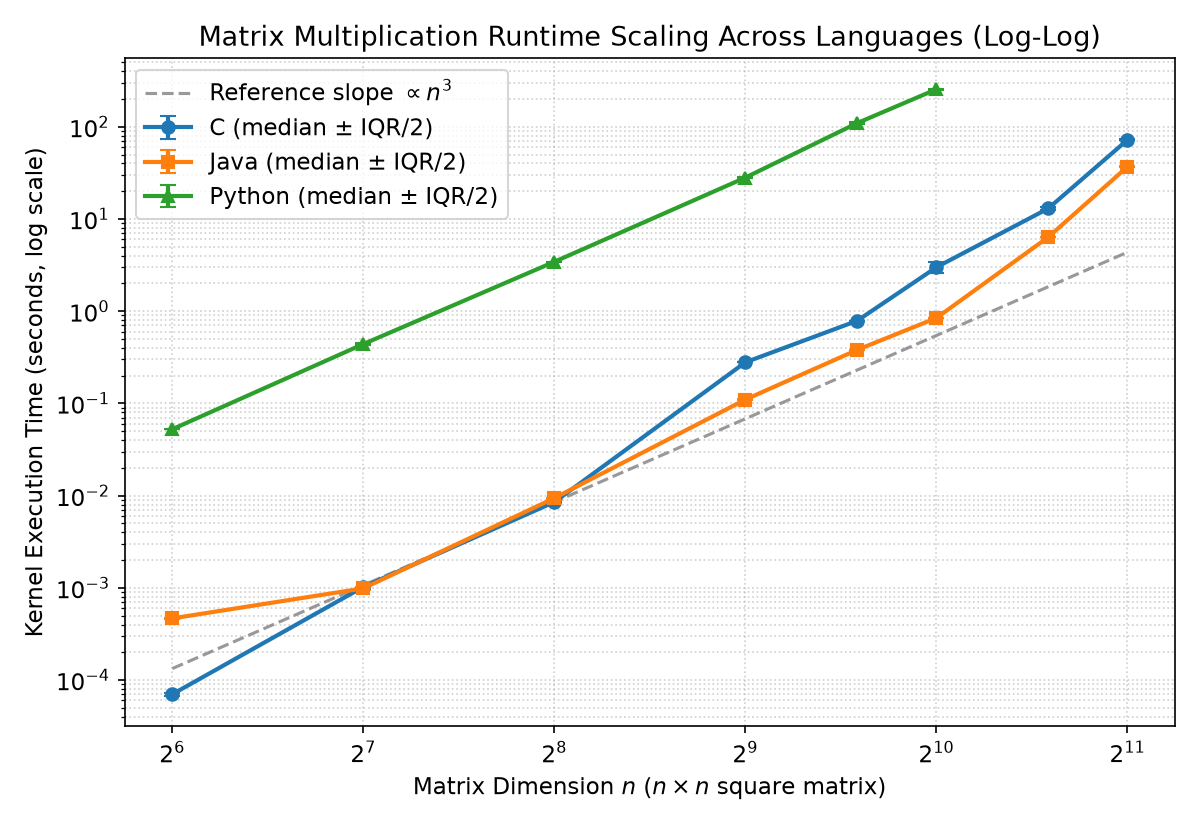
\includegraphics[width=0.75\textwidth]{results/log_log_runtime_scaling.png}
    \caption{Execution time vs.\ matrix size $n$ (log-log scale).}
    \label{fig:loglog}
\end{figure}

\begin{figure}[H]
    \centering
    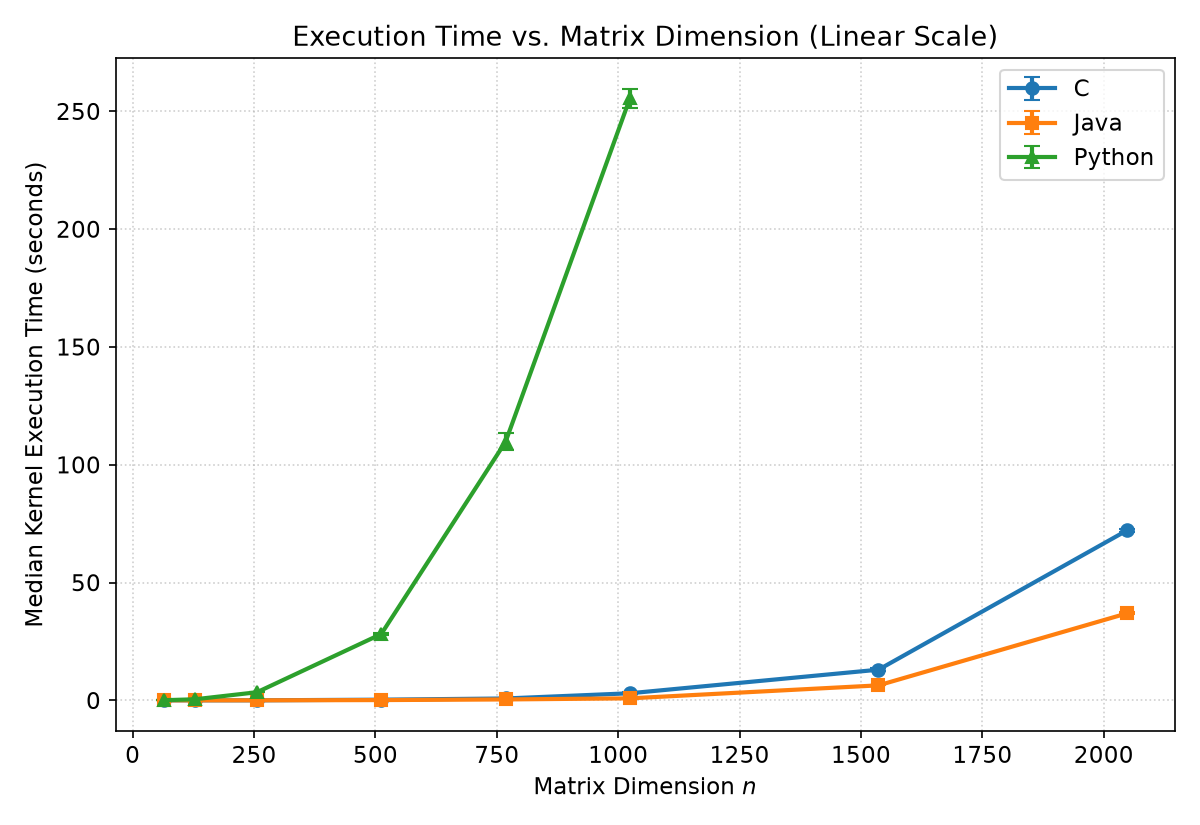
\includegraphics[width=0.75\textwidth]{results/linear_runtime_comparison.png}
    \caption{Execution time vs.\ matrix size $n$ (linear scale).}
    \label{fig:linear}
\end{figure}

\begin{figure}[H]
    \centering
    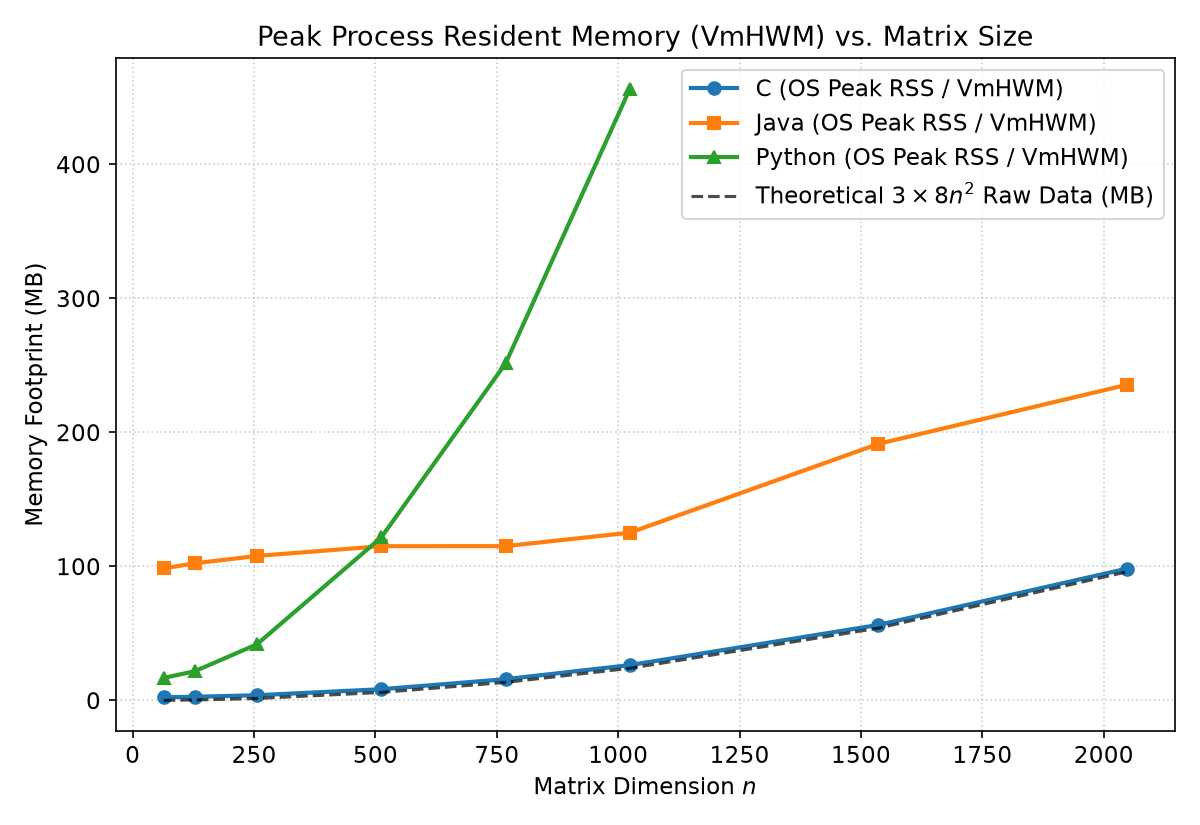
\includegraphics[width=0.75\textwidth]{results/memory_footprint_comparison.png}
    \caption{Peak resident memory (\texttt{VmHWM}) compared to theoretical matrix size ($3 \times 8n^2$).}
    \label{fig:memory}
\end{figure}

\section{Discussion}

\subsection{Execution Time Comparison}
As shown in Figure~\ref{fig:loglog}, all three implementations follow the cubic $O(n^3)$ trend. However, there are clear differences between languages:
\begin{itemize}
    \item \textbf{Python:} It is by far the slowest language (255.42 s at $n=1024$, compared to 2.999 s in C and 0.845 s in Java). Because Python is interpreted, each step of the loop has to access list objects and create float objects, taking around 200--240 ns per operation for all matrix sizes.
    \item \textbf{C vs.\ Java:} For small sizes ($n=64$), C is faster than Java (0.000070 s vs.\ 0.000466 s) because the matrices fit inside the fast L1/L2 CPU caches. However, for $n \ge 512$, Java is faster than C (0.845 s vs.\ 2.999 s at $n=1024$, and 36.92 s vs.\ 72.14 s at $n=2048$). In C, storing the matrix in a single 1D array and reading column $B$ by jumping $n$ positions causes many CPU cache misses, especially when $n$ is a power of two ($512, 1024, 2048$). Notice that in C, the time per operation drops from 2.082 ns at $n=512$ to 1.738 ns at $n=768$ (not a power of two). In Java, each row of \texttt{double[][]} is a separate object in memory and the JVM JIT compiler optimizes the loop at runtime, avoiding that cache problem.
    \item For $n=1536$ and $n=2048$, the matrices take 54 MB and 96 MB, which is larger than the 18 MiB L3 cache of the CPU, so both C and Java become slower per operation.
\end{itemize}

\subsection{Memory Usage and Limitations}
In Figure~\ref{fig:memory}, C uses almost the exact theoretical memory needed for the three matrices (100.75 MB Peak RSS at $n=2048$ vs.\ 98.30 MB theoretical). Java starts with a high base memory ($\sim 100.9$ MB at $n=64$) because the JVM reserves memory at startup (\texttt{-Xms512m}), although its used heap grows normally with matrix size. Python uses the most memory (467.4 MB Peak RSS and 104.5 MB in \texttt{tracemalloc} at $n=1024$, where the raw numbers only need 24 MB) because Python stores every float as a separate object in memory.

\textbf{Limitations:} The three memory tools (\texttt{VmHWM}, Java heap, and \texttt{tracemalloc}) measure different levels of memory and cannot be compared as identical metrics. Also, these results only reflect the basic \texttt{i-j-k} loop on a single thread; changing the loop order or using cache blocking in the next assignment will change the C and Java times.

\section{Conclusions}
\begin{enumerate}
    \item C, Java, and Python all follow the expected $O(n^3)$ time growth and produce the exact same numerical results across all tested sizes.
    \item C uses the least memory and is fastest for small matrices ($n \le 256$), while Java is faster for larger matrices ($n \ge 512$) in this unoptimized \texttt{i-j-k} test due to JIT optimizations and fewer cache conflicts.
    \item Pure Python is too slow and uses too much memory for large dense matrices (255.4 s and 467.4 MB at $n=1024$).
\end{enumerate}

\section*{References and Materials}
\textbf{Reproducibility Materials:} All source files (\texttt{src/}), validation data (\texttt{data/validation\_suite.txt}), raw measurements (\texttt{results/raw\_measurements.csv}), summary tables (\texttt{results/summary\_metrics.csv}), plots, and the script \texttt{run\_all.sh} are included in the repository.

\smallskip\noindent
\textbf{AI Usage Disclosure:} Gemini (Google) was used to help write the plotting script in Python (\texttt{matplotlib}), structure the bash automation script, and review the English text and \LaTeX\ formatting. All tests were run and verified locally by the author.

\begin{thebibliography}{9}
\bibitem{guide}
ULPGC Big Data Course, \emph{Individual Assignments: Matrix Multiplication Specification}, Academic Year 2026--2027.

\bibitem{pydocs}
Python Software Foundation, ``\texttt{time} and \texttt{tracemalloc} --- Python 3.14 Standard Library Documentation,'' 2026. [Online]. Available: \url{https://docs.python.org/3/}
\end{thebibliography}

\end{document}
